\begin{figure}
	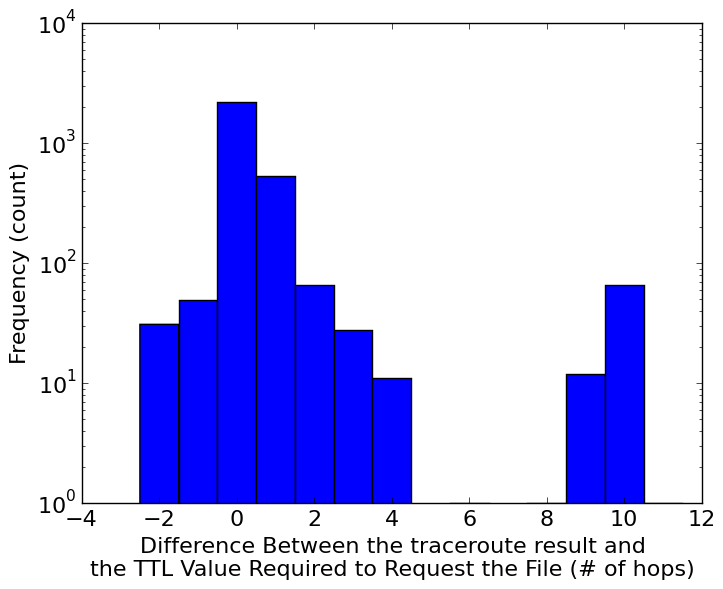
\includegraphics[width=\columnwidth]{figures/gcprobehist}
	\caption{
		A histogram showing how often a file request succeeded with a TTL value less than the number of hops to the server (as estimated by \texttt{tcptraceroute}~\cite{Toren2006}).
		A zero value on the x-axis represents files which were not received until the TTL value of the request was set to the result of the \texttt{tcptraceroute}.
		Larger values on the x-axis represent files which were received when the TTL value of the request was less than the result of the \texttt{tcptraceroute}.
		Negative values represent files which were not received until the TTL value of the request was set to be greater than the result of the \texttt{tcptraceroute}.
		Files which were not received even when the request was sent with a TTL value 3 greater than the \texttt{tcptraceroute} result are not shown.
	}
	\label{fig_gcprobehist}
\end{figure}